\chapter{Payment Feature}
\label{chap:payment-feature}

% Nomenclature - JSON?

\section{Sever Side Implementation}
\label{sec:server-side-implementation}

The greatest concern in implementing a payment feature for Synote is remaining PCI DSS compliant. To remove most of the burden and with the approval of our client Yunjia Li, Stripe was chosen as the payment gateway. Stripe also allows custom merchant forms which our client favours over redirection and generated forms.\\

\begin{figure}[!hbt]
  	\centering
 	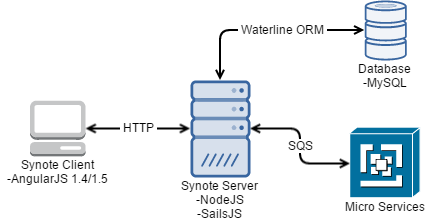
\includegraphics[width=0.78\textwidth]{synote-architecture.png}
  	\caption{Synote Architecture}
 	\label{fig:synote-architecture}
\end{figure}

\textbf{Figure \ref{fig:synote-architecture}} depicts Synote's existing architecture which uses Node.js (Node) and Sails.js (Sails) web frameworks on the server. Sails includes a powerful Object Relational Mapping (ORM) tool called Waterline to provide a data access layer to the underlying MySQL database.\\

As a custom merchant form is desired for gathering payment information, Stripe must be used to tokenize the payment data before it can be sent to Synote's server. As mentioned in \textbf{Section \ref{subsec:security}}, HTTPS is required for secure transmission of payment data over a network, so the first stage of integration is to use an HTTPS/SSL certificate to enable HTTPS communication. The resulting architecture is shown in \textbf{Figure \ref{fig:stripe-integration}}.\\

\begin{figure}[!hbt]
  	\centering
 	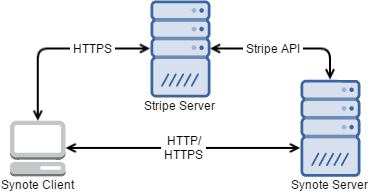
\includegraphics[width=0.7\textwidth]{stripe-integration.png}
  	\caption{Integrating Stripe}
 	\label{fig:stripe-integration}
\end{figure}

The first iteration of the payment feature requires simple functionality: A customer must be able to enter payment information to buy \texttt{X} amount of credits which will be stored against their Synote account, along with a record of the transaction. \textbf{Figure \ref{fig:simple-sequence}} shows the full sequence of events necessary to achieve this behavior, however, server side implementation concerns only what happens as a result of the \texttt{POST} action to Synote's server.\\

\begin{figure}[!hbt]
  	\centering
 	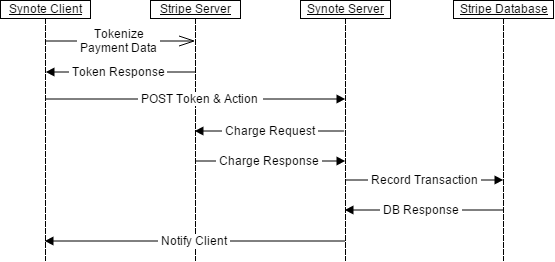
\includegraphics[width=\textwidth]{simple-sequence.png}
  	\caption{Sequence Diagram Of Simple Payment}
 	\label{fig:simple-sequence}
\end{figure}

Step one is to create the endpoint to which a Stripe token and any additional required information can be posted. Sails has an API called Blueprint which creates RESTful routes when an endpoint is created with a \texttt{model} and \texttt{controller}. Further routes can be added to the endpoint route through the concept of action routes, thus a \texttt{controller} file named \texttt{CreditHistoryController.js} containing an action route of \texttt{topup} exposes the route: \texttt{/credithistory/topup}.\\

Making charges against a token requires Stripe's API \cite{stripe-api} which can be added using the \texttt{require} keyword and must include a secret key provided by Stripe. Stripe's API lists examples of functions in Node, but in the form of callbacks. As covered in \textbf{Section \ref{sec:synote}}, the convention is to use promises in favour of callbacks which altogether results in code similar to \textbf{Listing \ref{lst:stripe-charge}}.\\

\hspace{0.1\textwidth}
\begin{minipage}{.76\textwidth}
\begin{lstlisting}[caption=Stripe Charge Promisified Example, label={lst:stripe-charge}]
var stripe = require('stripe')(StripeSecretKey);

return stripe.charges.create({
        amount: cost,
        currency: "gbp",
        source: token.id
});
\end{lstlisting}
\end{minipage}
\hspace{0.1\textwidth}

Information required to make a charge includes a single use token, charge amount and currency. The token and charge amount are provided in the \texttt{POST} from a client as a JSON object in the request (\texttt{req}) body. It is convention that a \texttt{req} is only processed within a \texttt{policy} and \texttt{controller}. Sails uses policies for authorization and access control such that each \texttt{action route} for each \texttt{controller} can be assigned one or more policies. As Synote uses Auth0 \cite{auth0} a policy called \texttt{hasJsonWebToken} exists to add a user's profile to a \texttt{req} which, aside from authorization, has the added benefit of providing a user's ID that can be used to determine which user is making a purchase.\\

\begin{figure}[!hbt]
  	\centering
 	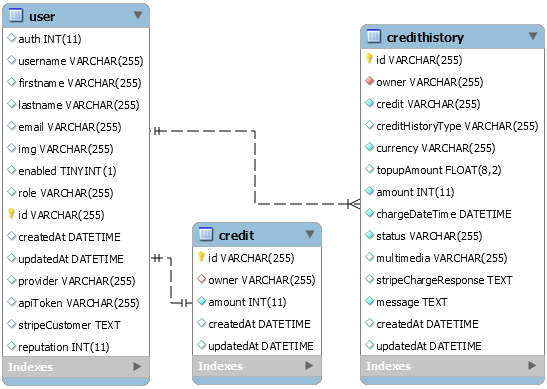
\includegraphics[width=\textwidth]{db-credit.png}
  	\caption{Credit \& Credit History Database Tables}
 	\label{fig:db-credit}
\end{figure}

The remaining task is recording the transaction and assigning purchased credits to a user. The setup for this task requires alteration to the existing database (DB), a Sails \texttt{model} and Waterline methods to interact with the DB. \textbf{Figure \ref{fig:db-credit}} shows the schema of the credit and credit history tables with their relations to the existing user table. Adding these tables to an existing database requires use of an SQL migration file as shown in \textbf{Listing \ref{lst:migration-file}}.\\

\hspace{0.1\textwidth}
\begin{minipage}{.72\textwidth}
\begin{lstlisting}[caption=Section Of Migration File: v0.9.0-v0.10.0.sql, label={lst:migration-file}]
DROP TABLE IF EXISTS `testing`;
CREATE TABLE `testing` (
  `id` VARCHAR(255) NOT NULL,
  `email` VARCHAR(255) NOT NULL,
  `role` VARCHAR(255) NOT NULL,
  `free` BOOLEAN DEFAULT TRUE,
  `createdAt` datetime DEFAULT NULL,
  `updatedAt` datetime DEFAULT NULL,
  PRIMARY KEY (`id`)
) ENGINE=InnoDB DEFAULT CHARSET=utf8;
\end{lstlisting}
\end{minipage}
\hspace{0.1\textwidth}

A section of the \texttt{model} file required for Waterline ORM to interact with the database is shown in \textbf{Listing \ref{lst:credit-history-model}}. Each attribute of the \texttt{model} is a one-to-one mapping with a field in the corresponding table, in this case \texttt{stripeChargeResponse} is shown with a type of \texttt{text} which can clearly be seen in the \texttt{credithistory} table of \textbf{Figure \ref{fig:db-credit}}. This field exists to store a record of the charge response from Stripe and contains redacted PCI DSS compliant information such as the last four digits of the charged card. Also of note in \textbf{Listing \ref{lst:credit-history-model}} are two examples of Waterline functions: \texttt{findOne} and \texttt{update} which in this instance are part of a hook to update the quantity of credits for a user after a purchase. These functions are a subset of the available functions to Create, Read, Update and Destroy (CRUD) DB records.

\begin{lstlisting}[caption=CreditHistory.js model file, label={lst:credit-history-model}]
module.exports = {
    attributes: {
		//Code omitted
        stripeChargeResponse: {
            type: "text",
            isTopUp: true
        },
		//Code omitted
    },

    afterCreate:function(history,cb){
      Credit.findOne({id:history.credit})
        .then(function(oldCredit){
          var newAmount = oldCredit.amount+history.amount;
          return Credit.update({id:history.credit},{amount:newAmount});
      }).then(function(newCredit){
        cb();
      }).catch(function(err){
        cb(err);
      });
    }
};

\end{lstlisting}

The second iteration of the payment feature requires extended functionality: A customer must be able to save payment information for faster future purchases. Stripe provides a method of saving payment data which encapsulates sources such as payment cards in a \textit{customer} object. The ID of a customer object can be used to charge a user's default payment source, or the combination of customer object id and source-data ID can be used to charge a specific card owned by a customer. Building on the first iteration and following the process above, server side implementation for saving cards and paying with saved cards involves:

\begin{enumerate}
	\item Adding action routes in the \texttt{CreditHistoryController.js} file to retrieve/delete cards
    \item Providing additional parameters in the \texttt{req} body JSON to indicate the Stripe token should be used to save the payment data
    \item Adding policies to secure the new routes
    \item Adding Stripe functions to save payment data in a Stripe customer object
    \item Updating the database schema using a migration file to store a Stripe customer object against a user
    \item Updating the relevant \texttt{model} to include the Stripe customer field
    \item Adding Waterline functions to CRUD Stripe customer records in the DB
\end{enumerate}

All of the Stripe and Waterline methods can exist in \texttt{CreditHistoryController.js} file, but this constitutes poor cohesion and it is convention to keep reusable functions in a \texttt{service} file to prevent repetition. Consequently all reusable Stripe functions are placed in \texttt{StripeService.js} and all reusable Waterline functions are placed in \texttt{ChargeService.js} for maximal cohesion. The resulting solution architecture is shown in \textbf{Figure \ref{fig:synote-stripe}}.

\begin{figure}[!hbt]
  	\centering
 	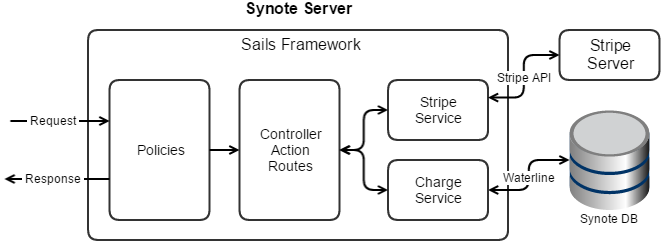
\includegraphics[width=\textwidth]{synote-stripe-overview.png}
  	\caption{Overview Of Synote-Stripe Architecture}
 	\label{fig:synote-stripe}
\end{figure}

\section{Server Side Testing}
\label{sec:server-side-testing}

\section{Client Side Design}
\label{sec:client-side-design}

\subsection{Screenshots}
\label{subsec:screenshots}

\subsection{Business Logic}
\label{subsec:business-logic}

\subsection{Diagrams}
\label{subsec:diagrams}

\subsection{Responsive Design}
\label{subsec:responsive-design}

\subsection{Validation Messages}
\label{subsec:validation-messages}
